\chapter{Suggested method for importing FKB into OpenStreetMap}
Proof of concept 

\section{Method - Microtasking?}

% Går tilbake til metodene, hva kan vi lære i Norge hvor vi ikke har Mapbox. Norske FKB er bedre enn de man har importert i andre land
% Er dette beste metode?
%Hvordan dele opp i tasking områder? telle antall hus. 50-30-20 hus innenfor hver task? Dette er en utfordring, men er utenfor scopet til oppgaven. Komme med noen tanker rundt hvordan det kan løses. 


\section{FKB to OSM tagging}
%Hvilke tagger skal brukes for hva
%Skal vi bruke relations med 3D støtte? 

An example of a area representation of a building feature type is shown in listing \ref{eq:buildingfootpr}. This can be used as the building footprint when converting FKB to OSM. This will create the 2D modeling. 

\lstset{
    language=XML,
    morekeywords={encoding,node, tag},
    label=eq:buildingfootpr,
    caption=Example of a area representation of a building feature type in SOSI. 
}
\begin{lstlisting}
.FLATE 715235:
..OBJTYPE Bygning
..KOMM 1601
..BYGGNR 182720836
..BYGGTYP_NBR 111
..BYGGSTAT TB
..KOPIDATA
...OMRÅDEID 1601
...ORIGINALDATAVERT "Trondheim kommune"
...KOPIDATO 20160502
..REF :166806
..NØ
703610900 55898600
\end{lstlisting}

Using figure \ref{fig:buildtypTrd} of the twenty most common building types in Trondheim, there are in total about 140 different types \cite{SOSI-sekretariatet}. Not all building types used in FKB can directly translate to OSM. In the taginfo web page users can search for values commonly used on the building key. The taginfo page was helpful when transferring the FKB building types over to building values in OSM. For instance, type 181 is garage, 111 is detached house (\textit{enebolig}) and 121 is house and are the three most common building types in Trondheim. A list of the 40 most common building types transferred into building values in OSM is in the appendix, table \ref{tab:fkbtoosmdel1} and \ref{tab:fkbtoosmdel1}. 

\begin{figure}[H]
    \centering
    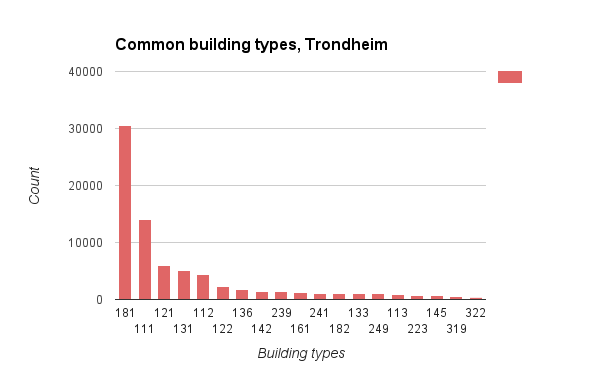
\includegraphics[scale=0.5]{figures/FixedByMe/buildtypestrd.png}
    \caption{20 most common building types in Trondheim, source: postgis query in the cadastre} 
    \label{fig:buildtypTrd}
\end{figure}

These values will represent the value for the building key given to the building feature type. The building feature in listing \ref{eq:buildingfootpr} will be given the value detached (building=detached).  


\section{Conversion using existing script}
% fkbbuilding.lua
%Lage utkast til en luafil, vise hvordan xml oppsettet blir 

The sosi2osm script was developed in 2013 by the github user Gnonthgol. It was created during the N50 imports initial stages.*%Finn kilden   
 The script is open source and the repository is available at Gnonthgol's GitHub account. The Sosi2osm repository do not have any documentation, the only available help is a wiki page who shortly explain how to install and run the code. It is very difficult to install, especially if you don't have a linux operating system. The script depends on fyba. A open source code distributed by the National Mapping Authority of Norway (Kartverket) to read and write SOSI files. Sosi2osm do not support SOSI files encoded in UTF-8. This is a challenge since FKB sosi files can be UTF-8 encoded.*%Er FKB alltid UTF8 eller bare i noen kommuner?
 This is a major drawback with this script. To test the script, after managing to install it correctly, the first step is to encode the FKB SOSI file into ISO8859-10. %Er alle SOSI filer i UTF 8 idag?

When running the script, input is a sosi file and a lua script. A new lua script is created for each dataset. In the N50 import they created one lua file for land cover (\textit{arealdekke}), there is also a lua file for address import. For testing the sosi2osm script I programmed a fkbbuilding.lua file. Adding values to the building key, which depend on the buildingtype code from FKB, I used table \ref{tab:fkbtoosmdel1} and \ref{tab:fkbtoosmdel1}. See listing \ref{eq:luabuldtype} for the code snip checking the building value. This code snip checks the $BYGGTYP\_NBR$ attribute value to determine the buildings particular usage. The building=* key-value pair will be placed on the buildings footprint, since only building feature in FKB has this attribute value. 

It is not possible to add height in ways and node representations. Another problem with the sosi2osm script is that it do not consider height values, creating one node for each north, east coordinate pair. If two crossing building lines have different height values they should not share the same node \cite{OpenStreetMap2015}. This is a problem, especially when considering 3D modeling of buildings. 


\section{How to map FKB buildings in 3D}
%Her kan jeg lage et eksempel på hvordan 3D bygg kan moduleres i OSM XML format. 
In order to create a XML representation capable of modeling FKB buildings in 3D, a standard approach should be developed. Members of the OpenStreetMap community, with interest in 3D mapping, started in March 2012 to unite all the separated approaches to model 3D buildings using OSM XML \cite{OpenStreetMapm}. They arranged workshops, which resulted in a suggestion for a simple 3D building schema. This is the approach mentioned in section \ref{buildOSM}. This approach is fairly easy to implement, if the building's roof shape is known. This is not the case for the FKB buildings, so the simple 3D building schema needs modification. Buildings in FKB is modelled with ridge and edge lines and they can be used to create 3D models, see the figures in section \ref{sec:FKBbuilding}. When using ridge and edge modeling, roof shape tags are ignored, meaning the shape of the roof is not needed. Collecting ridge- and edge-lines for one building, creating a way-representation for each line with roof:edge and roof:ridge key's on each. The way-tag representing the building outline, most often the roof-edge feature, holds the height and roof:height information.*%Funker ikke paa alle type bygninger, bare de som har en closed-way rundt hele omrisset
 The listing shown in \ref{eq:3D_fkbbuilding} creates a 3D representation of a house in OSM from FKB data. The house is shown in figure \ref{fig:3DFKBbuild}, using the JOSM editor to generate the code in listing \ref{eq:3D_fkbbuilding} and getting 3D visualization using the JSOM plugin kendzi3d. 

\begin{figure}[H]
    \centering
    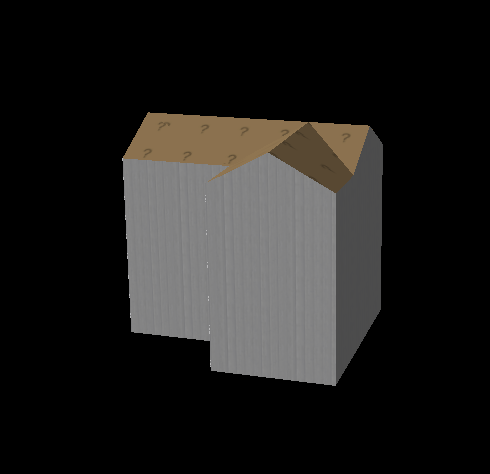
\includegraphics[scale=0.5]{figures/FixedByMe/3DFKBbuilding.png}
    \caption{3D representation of a FKB building, result of listing \ref{eq:3D_fkbbuilding}}
    \label{fig:3DFKBbuild}
\end{figure}

In OpenStreetMap, building height is the distance between the lowest possible position with ground contact and the top of the roof of the building, excluding antennas, etc \cite{OSMwikipage2016}. Height of buildings in FKB is height above sea level. This is a new challenge when mapping FKB buildings in OSM. In listing \ref{eq:3D_fkbbuilding} height above sea level is manually withdrawn from the height given from the FKB data. 

The approach described here do not work on all building types. 

%The participants on the workshop agreed on building outlines should be used for the most general area of a complex building and building parts used to describe the special parts with different heights or other attributes, etc. As mentioned in section \ref{buildOSM}, the building outline should be tagged with building=* and building parts with building:part=*. Building outline is either a closed way or a multi-polygon and represents the area of land covered by the union of all building parts, the building footprint \cite{OSMwikipage2016}. Attributes like address, name, height, etc. must be tagged on the building outline. The building outline is important because it provides the compatibility for 2D rendering software. 2D renderers ignore building:part=* tags and only displaying the building outline. A relation tagged with type=building should be used if there are more than  one building part. This groups the building outline and all building parts together, as mentioned in section \ref{buildOSM}. 

There are different tools developed to visualizing 3D buildings with data from OSM. A problem is that not all tools supports the different modelling. A list of which of them who supports the simple 3D building schema is located at the OSM simple 3D buildings wiki page, most tools accept this schema. 7 tools supports building:part=yes %http://wiki.openstreetmap.org/wiki/3D_Development/Tagging#Usage_Community
2D renderers ignore building:part=* tags, only displaying the building outline. %kanskje vise hvordan huset ser ut i demo.f4map.com?

An example of 3D building generated from FKB data is shown in listing xx. This use the simple 3D building schema. 



\section{Evaluation}

